\documentclass{article}
\usepackage{tikz}
\title{Basic Drawing Practice}
\author{Sumaiya Tabassum}
\begin{document}
	\maketitle
	\section{Draw Line}
	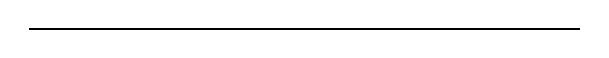
\begin{tikzpicture}
		\draw[thick, -] (0,0) -- (7,0);
	\end{tikzpicture}
	
	\section{Axis Line}
	\begin{tikzpicture}
		\draw[thick, ->] (0,0) -- (4,0);
		\draw[thick, ->] (0,0) -- (0,4);
	\end{tikzpicture}
	
	\section{Axis Line}
	\begin{tikzpicture}
			\draw[->] (0,0)--(4,0) node[anchor = north west]{x axis};
			\draw[thin, ->] (0,0) -- (0,4) node[anchor = south east]{y axis};
	\end{tikzpicture}
	
	\section{Circle}
	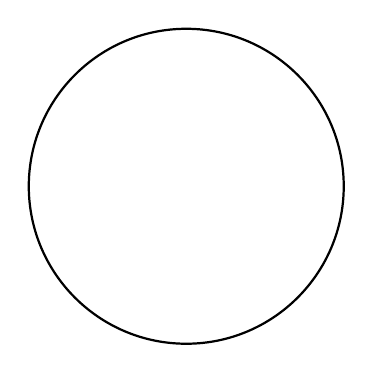
\begin{tikzpicture}
		\draw[thick] (0,0) circle(2);
	\end{tikzpicture}
	
	\section{Dashed Circle}
	\begin{tikzpicture}
		\draw[thick, red, dash dot] (0,0) circle(2);
	\end{tikzpicture}
	
	\section{Triangle}
	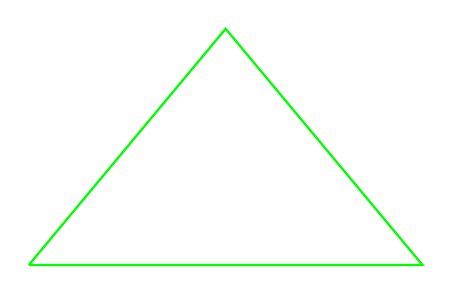
\begin{tikzpicture}
		\draw[thick, green] (0,0) -- (5, 0)--(2.5,3)-- (0,0);
	\end{tikzpicture}
	
	\section{Rectangle}
	\begin{tikzpicture}
		\draw(0,0) rectangle(2,2);
	\end{tikzpicture}
	
	\section{Parabola}
	\begin{tikzpicture}
		\draw(0,0) parabola(2,3);
		\draw(0,0) parabola(-2,3);
		\draw[dashed](0,-3)--(0,3);
	\end{tikzpicture}
	
	\section{Curved}
	\begin{tikzpicture}
		\draw(0,0) ..controls(0,2) and (4,0) ..(4,4);
	\end{tikzpicture}
	
	\section{Grid}
	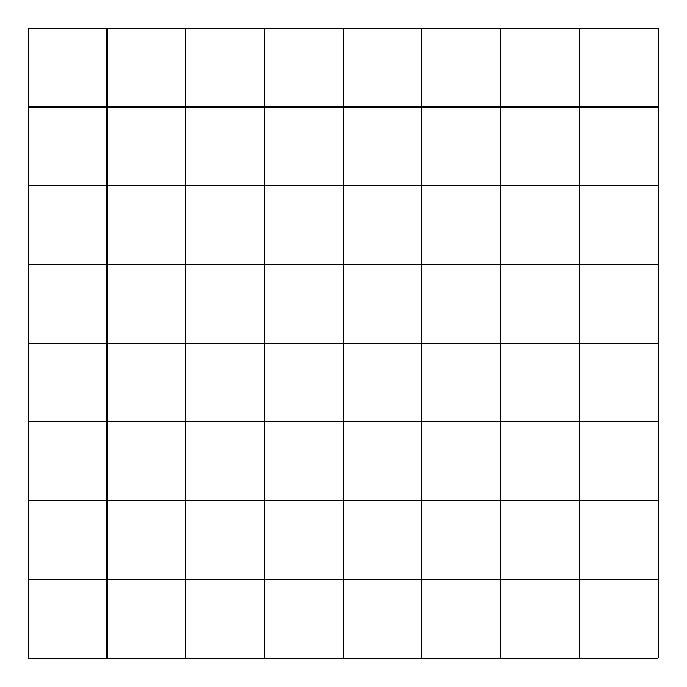
\begin{tikzpicture}
		\draw[step=1cm,black,thin](-2,-2) grid(6,6);
	\end{tikzpicture}
	
	\section{Arc:}
	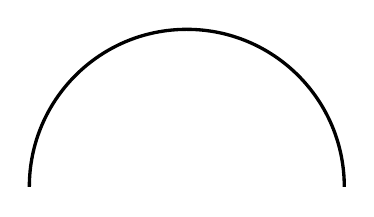
\begin{tikzpicture}
		\draw[very thick](0,0) arc(0:180:2cm);
	\end{tikzpicture}
	
	\section{Ellipse}
	\begin{tikzpicture}
		\draw(0,0) ellipse(3cm and 1.5cm);
	\end{tikzpicture}
\definecolor{darkgreen}{rgb}{0.0, 0.5, 0.0}	
	\section{Practice}
	\begin{tikzpicture}
		\draw[fill=darkgreen](-3,-2) rectangle(3,2);
		\draw[fill=red](0.15,0) ellipse(1.05cm and 1cm);
	\end{tikzpicture}
\end{document}